\section{Appendix\label{sec:appendix}}
\subsection{Notations}
We follow the ZOGY paper symbol notations. Frequency space quantities are
marked with \(\hat{\ }\), complex conjugation is marked by
\(\overline{x}\). Pixels of images are referred as functions
(\Cref{eq:img_func}). Expectation value of random variables are marked by
\(\langle\ \rangle\).
%
\par We use the terms \emph{image space} and \emph{Fourier- or frequency
  space} to refer to the discrete Fourier transform of images. \emph{Pixels}
may refer to either space depending on the context.
\begin{align}
x &= \{x(0), x(1), ... , x(n) \},\ x(n) \in \mathbb{R}\\
\hat{x} &= \{\hat{x}(0), \hat{x}(1), ... , \hat{x}(k) \},\ \hat{x}(k) \in
\mathbb{C}\\
\label{eq:img_func}
\end{align}
%
\subsection{Floating point values\label{sec:floating_point}}
The machine \emph{epsilon} is the smallest positive floating point value
where \(1 + \varepsilon \neq 1\). This is \(\approx 1e-16\) for double
precision.
%
\par The machine \emph{tiny} is the smallest positive floating point value
where the significand does not start with leading zeroes but the exponent is
the smallest representable. Going below this value the floating point number
looses significant digits and eventually rounds to exact zero. About
\(\mathrm{epsilon}\cdot\mathrm{tiny} = 0\).
%
\par Underflow to zero occurs around the order of the floating-point
\emph{tiny} value, we found, however, that this never practically
happens. In all our practical PSF transformation cases FFT values
cannot go a few orders below the floating-point \emph{epsilon} that is
several orders higher than the \emph{tiny} limit. This is
understandable if we consider that every pixel is a result of addition
operations, where the number of terms roughly equals to the number of
pixels in the image. As the PSFs are normalized, the zero frequency
value is always 1, which approximately sets the exponent of these
floating point values.
%
\par Furthermore, we usually zero pad a small PSF image to a larger image
size that creates a window function effect in the padded image. The
transformed image, therefore, have long oscillating tails in frequency space
and we found that all pixel (absolute) values remain a few orders even above
the epsilon threshold.
%
\subsection{Complex random variables}
%
\begin{equation}
\langle Z\rangle = \langle\Re(Z)\rangle + i\langle\Im(Z)\rangle
\end{equation}
%
\begin{equation}
\langle \bar{Z}\rangle = \overline{\langle Z\rangle}
\end{equation}
%
\newcommand{\Var}{\mathrm{Var}}
%
The variance and covariance of a complex random variable are defined as:
\begin{equation}
\operatorname{Var}(Z) \in \mathbb{R} \equiv \langle\abs{Z-\langle Z \rangle}^2 \rangle =
\langle\abs{Z}^2\rangle - \abs{\langle Z \rangle}^2
\end{equation}
%
\begin{align}
\operatorname{Cov}(X, Y) &\equiv \left\langle\left(X - \langle X \rangle\right)
\overline{\left(Y - \langle Y \rangle\right)} \right\rangle
= \langle X\bar{Y} \rangle - \langle X \rangle \overline{\langle Y \rangle} \\
\operatorname{Cov}(X, X) &= \operatorname{Var}(X)
\end{align}
%
\subsection{Discrete Fourier transformation normalization convention}
\par There is a freedom how normalization factors are placed in the
forward and inverse Fourier transforms.  This scales the individual
values of frequency components compared to corresponding pixel space
values. Usually, we do not need to worry about these scalings as the
forward and inverse operation factors cancel out. However, certain
frequency space relations change in their form if the normalization
convention changes, most importantly for us, the expression of the
convolution theorem changes.
%
The definition of DFT usually has the following normalization convention:
\begin{equation}
\hat{X}(k) = \mathcal{F}[x](k) \equiv \sum_n x(n) e^{-i\frac{2\pi}{N}k\cdot n}
\end{equation}
%
\begin{equation}
x(n) = \mathcal{F}^{-1}[\hat{x}](n) \equiv \frac{1}{N}\sum_k \hat{x}(k)
  e^{i\frac{2\pi}{N}n\cdot k}
\end{equation}
In this convention, the convolution theorem (and its dual) looks like:
\begin{equation}
\mathcal{F}[x \otimes y] =  \hat{x} \cdot \hat{y}
\end{equation}
\begin{equation}
\mathcal{F}[x\cdot y] = \frac{1}{N} \hat{x} \otimes \hat{y}
\end{equation}
Also:
\begin{equation}
\mathcal{F}[x](0) = \sum_n x(n)
\label{eq:X0sum}
\end{equation}
These relations change with factors of $\sqrt{N}$ if the transform
normalization changes. We must be sure that the correct convention is used
by numpy. This is the default as of v1.18.
%
\subsection{Noise variance properties in frequency space\label{sec:noise_freq_space}}
%
\par Let's take a look at the covariance of the Fourier transform of zero
expectation value pixels The complex covariance can be written as:
\begin{equation}
\begin{split}
\left\langle \hat{x}(k) \overline{\hat{x}(j)} \right\rangle =
\left\langle \sum_{n=0}^{N-1} x(n) e^{-i\frac{2\pi}{N}kn}
 \sum_{l=0}^{N-1} \overline{x(l)} e^{i\frac{2\pi}{N}jl} \right\rangle = \\
\sum_{n,l=0}^{N-1} \left\langle x(n)\overline{x(l)}\right\rangle e^{-i\frac{2\pi}{N}(kn - jl)} =
\sum_{n=0}^{N-1} \sigma(n)^2 e^{-i\frac{2\pi}{N}(k-j)}
\label{eq:freq_cov}
\end{split}
\end{equation}
%
\par If \(k=j\), we get the variance at each frequency. From the last
expression in \Cref{eq:freq_cov}, we can see that the variance is the same
at all frequency and it is the sum of the individual pixel
variances. Considering the normalization in the forward and inverse Fourier
transformation, we can think of this as the average of the individual pixel
variances, too.
%
\par This implies that using the average value of the variance plane as the
variance in frequency space is actually not an approximation but the exact
value.
%
\par If \(k\neq j\), but the individual pixel variances are equal, then the
phase factors in \Cref{eq:freq_cov} average out and we get that the
covariance in frequency space is zero between different frequencies. As a
similar expression and argument can be written for the pseudo-covariance, we
receive that any two different frequencies are uncorrelated. This is the
well-known relation that the Fourier transform of white noise is white noise. If
\(\sigma_n\)-s are not equal however, the phase factors won't average to
zero. Spatial variations of pixel noise introduce correlation in frequency
space noise. The correlation in frequency space encodes the spatial
distribution of \(\sigma_n\) values in image space.
%
\par We note that this is the case if we add zero padding to the
image, because the zero padding can be seen as pixels with zero sigma
noise. Also, if we change the correlation between frequencies by
multiplying with frequency-dependent factors, this implies a spatial
change of noise in image space, following the convolution
theorem.
%
\par Finally, let's consider a white noise image that got convolved by a kernel
image. From the convolution theorem, we get that in frequency space the
variance becomes frequency-dependent, but different frequencies remain still
uncorrelated.
%
\par We summarize these noise transformation properties in
\Cref{tab:freq_noise}, noting the duality of variances values and
correlation between pixels in image and frequency spaces. Our understanding
is that correlated noise in image space can be decorrelated by scaling in
frequency space so that all components have the same variance. This is one
of the key ideas in the ZOGY difference image construction, that one square
root of the likelihood variance weight can be assigned to the proper
difference image, so that its noise gets whitened (decorrelated). (The other
square root is part of the difference image PSF.)
%
\par The change of the spatial distribution of pixel sigmas follows the overall
convolution (like \(c_n, c_r\)) of the original uncorrelated images. If
furthermore, per pixel variances are uniform across the image, then the
whitening restores uncorrelated white noise across the image.
%
\begin{table}[h]
\begin{center}
\begin{tabular}{c|c}
  image space & frequency space \\
  \hline
  white noise & white noise \\
  \parbox{3in}{different variance values in uncorrelated pixels} &
  \parbox{3in}{same average variance at all frequencies
    but correlation in noise between different
    frequencies}
  \\
  \parbox{3in}{same variance but correlated pixel noise due to
  convolution operation} & \parbox{3in}{different variances at frequencies but
                 noise between frequencies are still uncorrelated} \\
\end{tabular}
\end{center}
\caption{\label{tab:freq_noise}Summary of image space and frequency space
  noise properties.}
\end{table}
%
\subsection{The resolution of DFT space\label{sec:dft}}
\par Finite DFT transforms N pixel into N pixel in frequency space. The
covered frequency range always goes from -1/2 through zero to \(\frac{1}{2}
\frac{1}{\mathrm{px}}\) frequencies but the resolution depends on the number
of input pixels (\Cref{fig:dft_sampling}). As conservation of information,
the N resulting frequencies can distinguish exactly N spatial positions. The
same concept is described by the interpretation that finite DFT always sees
the input as if it were periodic, giving the same result as if the input
were repeating in every N pixels. This also means that when we make a
frequency space manipulation we must see not only the input image or kernel
but the results as well to be periodic back in image
space.\footnote{\Cref{fig:dft_sampling} source:
  \texttt{https://en.wikipedia.org/wiki/File:Fourier\_transform,\_Fourier\_series,\_DTFT,\_DFT.svg}}
\begin{figure}[h]
\begin{center}
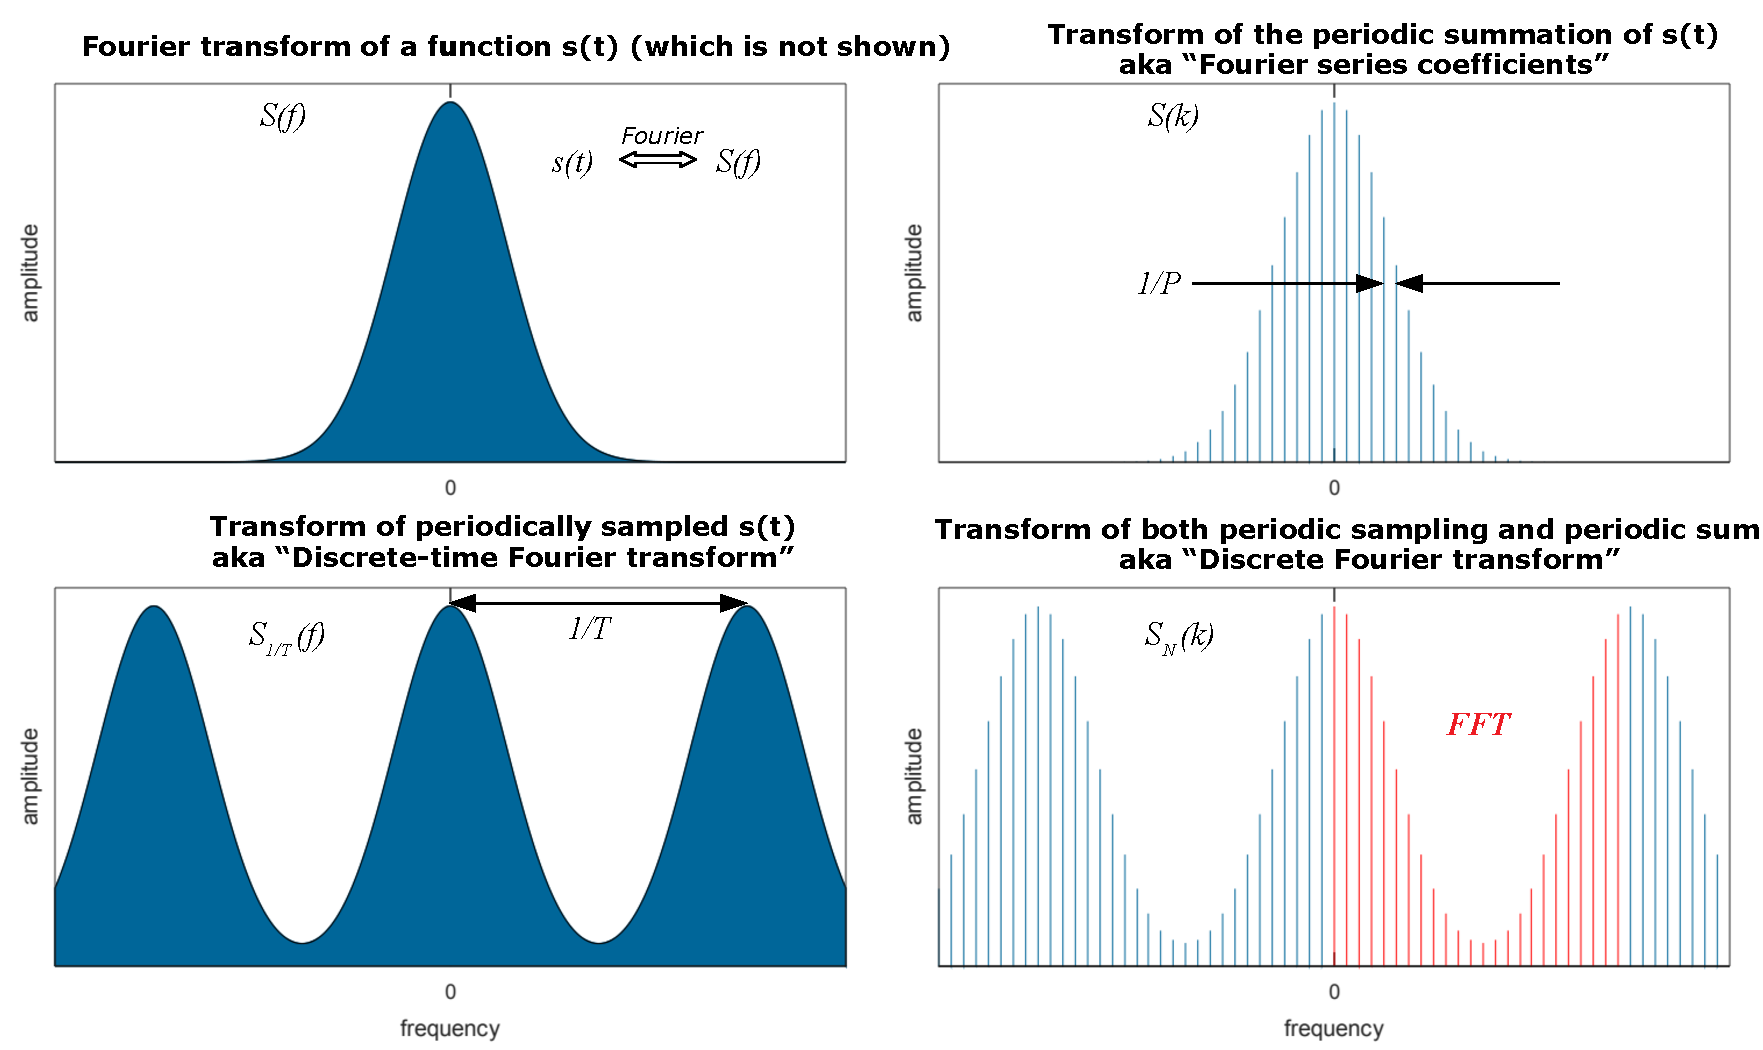
\includegraphics[width=5.5in]{fig/dft_sampling.pdf}
\end{center}
\caption{\label{fig:dft_sampling}Overview of sampling and periodicity
  effects in frequency space. Given the Fourier transform of a
  function (top left), sampling it every T time may cause a change in
  the frequency space values according to the sampling theorem (bottom
  left). This is called aliasing, in the bottom left panel, the
  minimum value shown is different from the top left panel. If the
  function is periodic, the frequency space values reduced to discrete
  values as well (top right). DFT/FFT combines the two concepts
  (bottom right). Considering unit pixel size, the FFT space always
  goes to 1/2 frequency with a resolution of 1/N. Figure source:
  Wikipedia:Discrete Fourier transform}
\end{figure}
%
\subsection{Zero padding in FFT frequency space\label{sec:zeropadS}}
%
\par While in image space convolution operations can have their own
way of handling edges, in Fourier space, multiplication always
corresponds to the circular boundary conditions in image space.  If we
want to implement a convolution without circular boundary
conditions that we want to calculate in frequency space,
we need to pad the images by extra edge pixels to avoid the
reappearance of values from the opposite side.
As we saw in \Cref{sec:patterns}, numerical artifacts in the matching
kernels cannot be bounded well in image space, they fill the full area
independently of the padding size. Therefore we cannot practically perform
the kernel matching convolutions in image space.
%
\par In the previous section, we also saw that a zero-padding violates one
of the ZOGY assumptions: that frequencies are independent and log
likelihoods can be calculated from them by simple addition. Is this a
significant inaccuracy in the score image?
%
\par Let's assume for a moment that the image background is extended in a
sourceless way with white noise. In this case, all the assumptions of the
detection statistics derivation hold thus we get \Cref{eq:Shat}. This is a
usual convolution expression in image space and at any pixel its value
depends only from the half \(P_d\) size neighboring area. If \(P_d\)
significant values are located in about the same square size as the original
PSF size then the affected edge area also remains the same. If the PSF
contains edges, however, \(P_d\) can be significantly bigger in size. Zero
padding adds pixels to an image that, from a noise model perspective, all
have a noise variance of zero. By padding the input images with zeroes, the
pixel variance of the difference image and, in a smaller edge region, the
score image variance will decrease. It is unclear whether scaling the score
image \(S\) with its variance plane satisfactorily corrects for this
effect. Nevertheless, this correction term is listed as a suggested
rescaling of the score image in the ZOGY paper Section 3.3. Beside this
correctional approach, we propose the implementation of padding with the
model white noise instead of constant zeroes in the future.
%
\subsection{Sampling}
\par It can be shown that Gaussians with \(0.95 < \sigma\), are well
sampled in the sense that \(3\sigma\) of their Fourier
transform Gaussian fit up to the 1/2 frequency limit. For
\(5\sigma\) fit, this is \(1.59 < \sigma\).

